\section{Work done to date}
\protect\label{section:workdonetodate}

The following outlines the work done to date.

\subsection{Software tools}
\protect\label{section:softwaretools}

In order to manage the large number of files, I set up a database using MySQL
and a Python library and tool set to access this conveniently. The database is
used to to manage records of each observation, the daily flat and bias files
taken, records of objects in the vicinity of each target with relevant data,
where objects were found in the images and ADU calculation results with
uncertainties. Most relevant FITS files are stored in the database but the
toolset created transparently fetches other FITS files as required.

\subsubsection{Display and analysis tools}
\protect\label{section:displayanaltools}

The contrast on the images is poor and I was unable to obtain any useful
photometry from standard image analysis software. I worked mainly with 
\textit{AstroImageJ} from which Fig. \ref{fig:aijimage} is derived. The
corresponding image from the software I developed is in Fig.
\ref{fig:myimage}.\footnote{I also tried \textit{AperturePT} before it ceased to
be usable on the Linux platform I was using, \textit{DS9} and the GAIA tool.}

The only way it appeared possible to proceed was to write my own display and
analysis software, from which the figures shown herein were derived. This finely
divides ADU counts into 16 different greyscales (with provision to increase
this to up to 32 greyscales). Pixels are assigned a given greyscale based upon
whether they fall within one of a set of percentiles.

With only a handful of the images could I make \textit{AstroImageJ} find the
target and after that only a handful of other objects, those having set the maximum
difference in flux to be 10,000\% or more of the brightest object using the
menus. When the objects were found, the ADU counts were comparable, well within
the same order of magnitude with the ones detected by my software.

\begin{figure}[!htbp]
\begin{center}
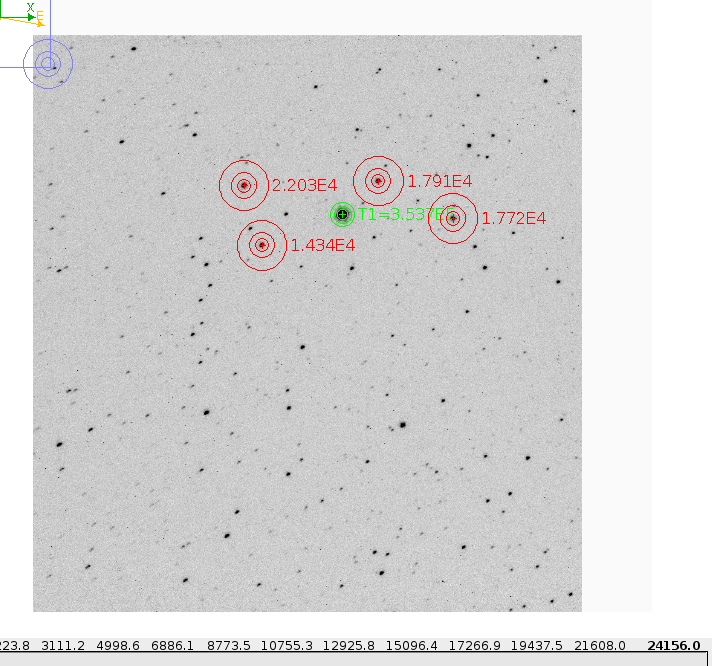
\includegraphics[scale=0.40]{images/AIJsnap.png} \\
\vspace{-.5cm}
\end{center}
\caption{This shows the display in \textit{AstroImageJ} of the observation of
{\ross} at 02:04:10 on 31 October 2021 in the \texttt{r} filter. The three
brightest objects together with the target gave been highlighted. However the
software was not able to find the objects on the image for this observation.}
\protect\label{fig:aijimage}
\end{figure}

\begin{figure}[!htbp]
\begin{center}
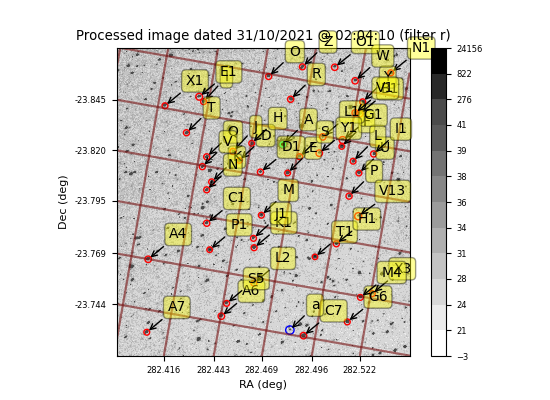
\includegraphics[scale=0.80]{images/myimage.png} \\
\vspace{-.5cm}
\end{center}
\caption{This shows the same display as Fig. \ref{fig:aijimage}, namely of
{\ross} at 02:04:10 on 31 October 2021 in the \texttt{r} filter using my
toolset with the first 10 brightest objects highlighted out of a total of 274
found. Labels are assigned from \textbf{A} through to \textbf{Z} and then
\textbf{A1} through to \textbf{Z1} etc in order of decreasing brightness on
average throughout the images.} \protect\label{fig:myimage}
\end{figure}

It proved that most of the objects found in the GAIA database and other sources
and with details copied across, nearly 60\%, had average of less than 1,000 ADU
counts above the sky level of $50 \pm 10$ ADU counts. Only 0.5\% of the objects,
always including the target object which was always well above 200,000 counts
for all but the poorest images, approximately 9 in total for the best {\ross}
images, slightly more for \prox, slightly less for \bstar, had ADU counts of 100
times the sky level and of those few frames had all of these due to differing
areas of the sky being covered by different frames.

\subsection{Master calibration files}
\protect\label{section:masterbiasflat}

In order to address the matters such as those referred to in Section
\ref{section:mattersaddressed} above, a study was made of the master bias and
flat files supplied. The main problem proved to be that the number of daily bias
or flat files going to make up the master files is not consistent, month by
month. Each master file is made up entirely from the daily files for the
calendar month concerned, which may vary considerably in number and criteria for selection.

Also some of the statistics for selection of daily files, notably the flat
files, are incorrectly calculated and/or stated.The master bias
files, as constructed, include extreme values for some pixels which cause
values for the image files to go negative when the bias file is subtracted as
no account is taken of noisy or unreliable pixels.

I also disagree with the method of calculating the master flat files, this is
because the daily flat files consist of sets of 3 in decreasing light and the
median value is taken, the result being then normalised. This causes the
benefit of the brighter flat files, with their better signal to noise ratio,
to be ignored in addition to the other ones.

% \begin{figure}[!htbp]
% \begin{center}
% 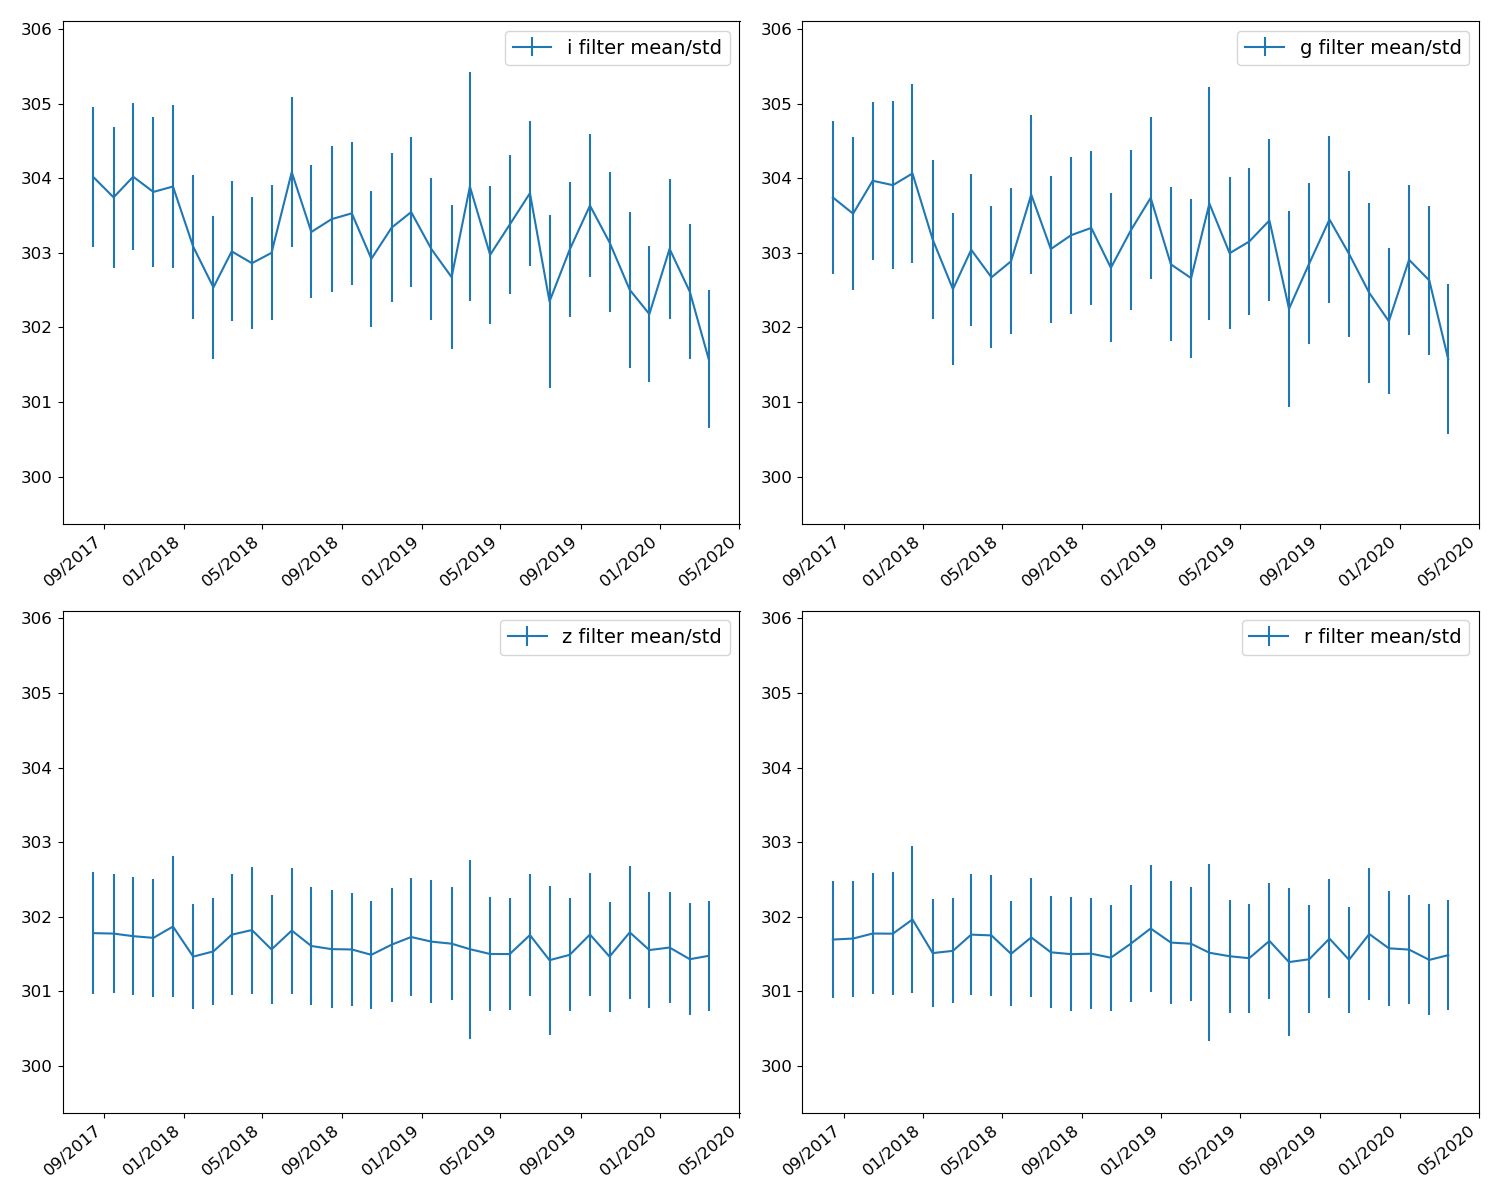
\includegraphics[scale=0.4]{images/mastmeanbias.png}
% \end{center}
% \caption{This illustrates the mean and the standard deviation of the values in
% the master bias files from July 2017, when {\rdwarf} targets were first
% observed, until March 2020.}
% \protect\label{fig:mastmeanbias}
% \end{figure}
I therefore decided to construct alternative ones from the daily bias and flat files
provided.

A key element in this was to construct the files using a rolling ``window'' of
the same number of daily files centred on the relevant date. This made a
substantial difference to the resulting master files, all of the variations
% seen in Fig. \ref{fig:mastmeanbias}
from month to month were eliminated and the resulting files were very similar.

\subsubsection{Defective or unreliable pixels}
\protect\label{section:badpix}

I undertook a study of all the files, flat files, bias files and observation
files to determine whether any pixels in the CCD array could be counted as
``bad'' or unresponsive, had particularly high mean values or large standard
deviation. The literature varies somewhat on how bad pixels are defined or
determined.

\Notnow{Of recent papers, \citet{allers20} define bad pixels as ``dead'' pixels or pixels
with an uncertainty in the flat fields of over 10\%. In \citet{piskunov20} bad
columns in the CCD used are first identified and eliminated and then an
iterative procedure is adopted to effectively assign weights to each pixel. In
\citet{bongiovanni19} a procedure based on constructing two composite flat
fields from low and high counts and regarding as bad the pixels where the ratios
differ by more than 15\%. In \citet{belli18} a bad pixel mask is constructed by
selecting pixels in the flat fields with very low counts and those in the dark
frames with very high counts (but the criteria for ``low'' and ``high'' counts
in those files are not defined). In \citet{briesemeister18} pixels in the
constructed flat fields with values less than 0.5 or greater than 1.5 are
considered to be bad.

A comprehensive study of the quality of pixels is described in the
recently-published \citet{maslennikova20}. Pixels are described as
\textbf{Normal}, \textbf{Cold}. \textbf{Warm}. \textbf{Dead}, \textbf{Hot} and
\textbf{Inverse} according to the responses. The pixels on the ROSS2 telescope
CCD do not fit neatly into these brackets, apart from the \textbf{Normal} ones.}

For the purposes of this study, it was clear that most of the pixels could be
described as acceptable with various degrees of noise, some extremely noisy.
There were a few, of the order of 25 pixels spread over the used area of the
array, which could be described as bad, in that no reliable result could ever be
obtained.

There were various examples of cosmics or other phenomena accepting individual
pixels randomly. In only rare cases would this contaminate the analysis.

It is straightforward to interpolate over the relevant pixels. There are a few
places where there are strings of adjacent noisy or consistently high pixels,
but these almost entirely affect columns in the CCD, the worst example can be
found in the area used for the \gfilter, seemingly as the CCD is read out by
columns, so adjacent pixels on the same row have to be used for interpolation.

\subsubsection{New master flat and bias files}
\protect\label{section:newmastfb}

With appropriate adjustments for the defective pixels as described above, it
proved straightforward to construct new master bias files using a  ``rolling
window'' centred on the date required. I constructed standard deviations for
each individual pixel, so each master bias and flat file consists of two planes,
one giving values for each pixel and the second giving the standard deviations.
These are combined where appropriate using the rules for combination of errors.

I made a study of the linearity using the daily flat files and found that the
CCD was could be regarded as linear if flat files were restricted to those
having ADU counts between 5,000 and 62,000. This issue must be returned to for
the observation files themselves, as most of the objects have ADU counts much
lower than 5,000.

This resulted in a much more satisfactory set of master bias and flat files and
it was possible to much more confident of the uncertainty of values on a
per-pixel basis. The combination of the flat files using a weighted
geometric mean, included many more of the brighter files, with their higher
SNR, giving them priority over the darkest files, whilst still obtaining some
benefit from the latter.

When the object ADU counts from {\rem} images are computed from the images, the
standard deviations for each individual pixel in the image are combined into an
overall standard deviation for the ADU count for the relevant object.

\subsection{Finding and identifying objects}
\protect\label{section:findingidentify}

I tried various strategies for locating object images in the frames. First I
looked for peaks in the frames, but due to the low ADU count from most of the
objects, it was hard to do this reliably without being confused by spurious
peaks on the CCD.

What proved more successful was to list and retain a database of possible
objects in the neighbourhood of the target objects using GAIA DR3 of magnitude
up to 19, which was the limit which the {\rem} telescope could detect.
Where alternative shorter names than ``GAIA DR3 nnnnnnn'' were available from SIMBAD
and other sources, then these were used in preference. Bearing in mind the
resolution of the {\rem} telescope of around 0.6 arcsecond, objects closer together than this
distance were eliminated, as were objects with irregular profiles and one marked
as variable.

The magnitudes in various bands are all noted in the database records, but these
were mainly used as a guideline where there was ambiguity in distinguishing
close but not overlapping objects. Aperture sizes were calculated by fitting a
Gaussian to approximate the PSF and taking the mean over the dataset of
acceptable images.\footnote{Other profiles, notably Lorentz, were tried but
this, although in some cases fitting rather better, made so negligible a
difference overall that it did not seem worth pursuing.} This works better with
some frames, such as in Fig.
\ref{fig:goodfit}, then others, such as Fig. \ref{fig:badfit}.

\begin{figure}[!htbp]
\begin{center}
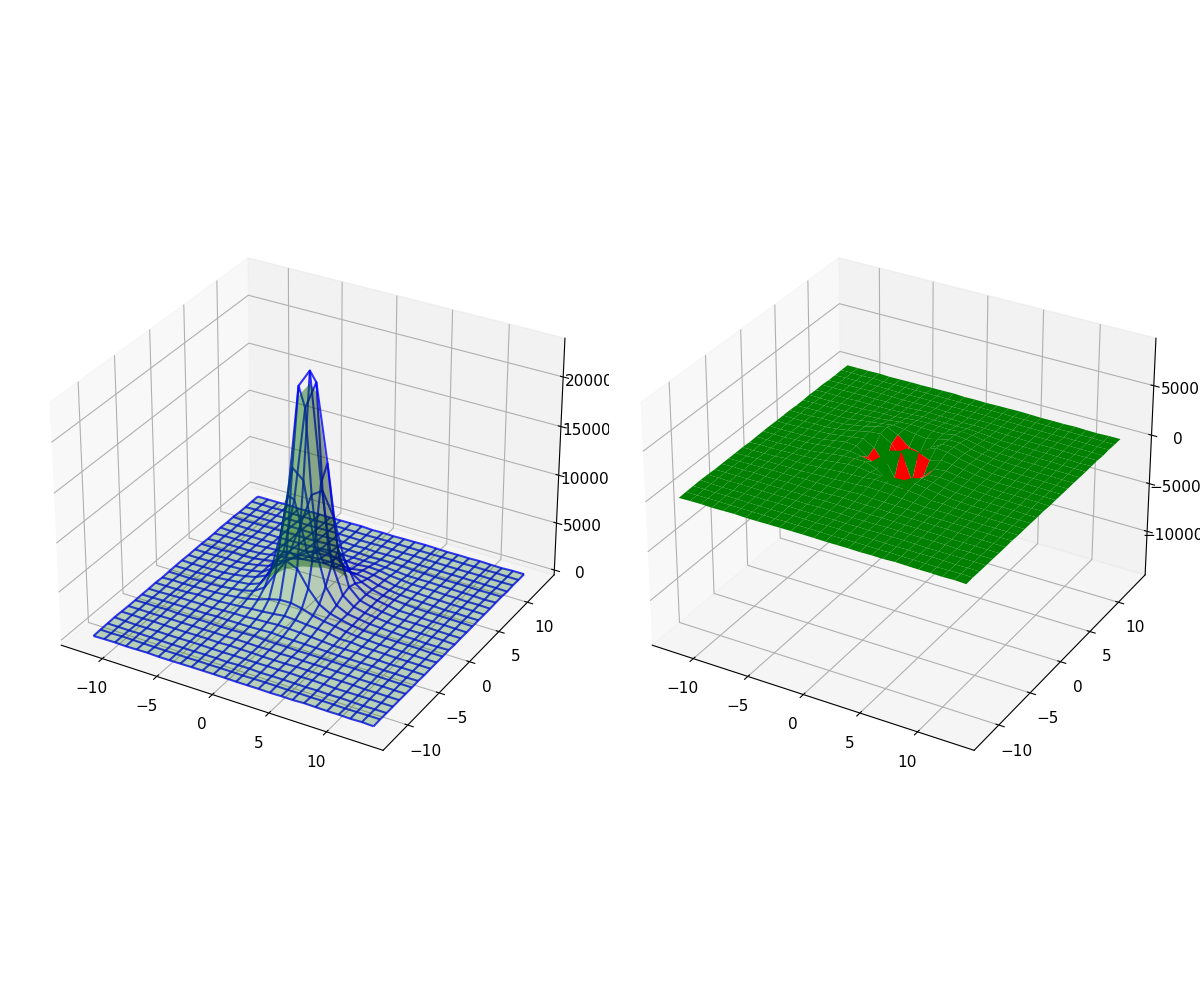
\includegraphics[scale=0.40]{images/goodfit.png} \\
\vspace{-.5cm}
\end{center}
\caption{This shows the profile and the fitted
Gaussian for the observation of {\ross} taken on 26
April 2019 at 08:54:03 with the \texttt{r} filter. The right
hand image shows the differences between this and
the actual flux, positive values in green and
negative in red. Air mass for this was 1.0085.}
\protect\label{fig:goodfit}
\end{figure}

\begin{figure}[!htbp]
\begin{center}
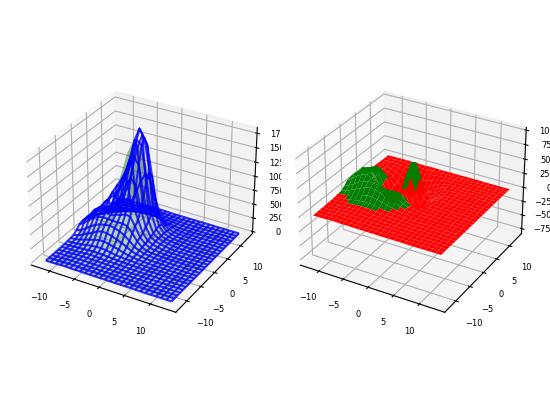
\includegraphics[scale=0.90]{images/badfit.png} \\
\vspace{-.5cm}
\end{center}
\caption{This shows the profile and the fitted
Gaussian for the observation of {\ross} taken on 16
September 2019 at 03:39:47 with the \texttt{r} filter. The right
hand image shows the differences between this and
the actual flux, positive values in green and
negative in red. Air mass for this was 1.5665.}
\protect\label{fig:badfit}
\end{figure}

There remains considerable work in finalising the optimal aperture sizes for
each objects, particularly with {\prox} and {\bstar}. It may be necessary to
calculate them individually for each frame, especially for the fainter objects.

The best frames contain over 200 possible reference stars for the best
examples, more for {\prox} and less for {\bstar}. Average frames contain up to
30 or so. Any with less than 30 are rejected as too poor.\footnote{This figure
is subject to amendment, currently the rejection is binary, but there is
provision for a ``quality'' marker enabling frames to be partially used where appropriate.}

\subsection{Calibration of reference stars and ADU counts}
\protect\label{section:calibrationrefstars}

As previously noted, not all the frames contain the same reference stars, or
have the same orientation, some are rotated by 90\degree or 180\degree relative to others. The
target object may be off-centre by varying amounts and in varying directions and
different reference objects appear in different frames, or are too close to the
edge in some cases, where vignetting or similar reduces the accuracy, to be
usable. Only a small handful (single figures) of brighter objects appear in
nearly all the frames and none, other than the target, appear in all of the
frames.

After some experimentation with strategies for computing and calibration of the
objects, the most promising strategy emerged as being for each filter.

\begin{enumerate}
  \item Compute the ADU count and standard deviation for each object in each
  frame.
  \item Compute the mean ADU count and corresponding standard
  deviation for each object. Clearly strongly variable objects previously missed can be weeded out
  at this stage.
  \item For each observation, perform a linear regression fit of the calculated
  ADUs for each object other than the target in the frame to the mean ADUs.
  \item Apply the fit backwards, propagating the standard deviation, to the
  calculated ADUs for the target on the frame and compare with the mean ADUs for
  the target to give the variation from the mean of the target for that frame.
\end{enumerate}

This technique proved very successful, in most cases the correlation of the
linear regression was better than 95\%, and proved insensitive to what set of
reference stars were available on a particular frame. However, as the targets
are very much brighter, by a factor of 100 or more, than the majority of the
reference stars, this linear regression technique involves a considerable
extrapolation to arrive at a calibrated ADU count for the targets.

Further, the ADU counts for the less bright objects are well below the lower
limit of linearity of the CCD of 5,000 mentioned for the flat files in Section
\ref{section:findingidentify} and this therefore needs to be returned to, in
order to improve the accuracy.

\subsection{Results for \ross}
\protect\label{section:resultsross}

The results for {\ross} are set out in the draft paper attached to this report.
but in summary the data sources referred to in papers which mentioned
measurements for {\ross} were studied and a rotation period of $2.87 \pm 0.01$
days was confirmed consistently.

After processing the data using the modified bias and flat files and processing
the counts relative to the reference stars as described above in Section
\ref{section:calibrationrefstars}, the period of 2.87 days was clearly extracted
from the data.

This confirms that there is viability in the methods used in terms of recovering
the rotation period for \ross. More challenging may be that for \bstar, where
the number of observations is less and also the number of reference objects.

\subsection{Problems with light curves for \ross}
\protect\label{secion:rossprobs}

There appears to be a problem with many of the observations for \ross, in that
there are huge swings seem to be observable in the calibrated flux within the course of a
few minutes. This is illustrated in the light curve shown in the draft paper
reproduced in Fig. \ref{fig:rossallcurve}. An example of the wildest set of
swings is seen in the September 2019 period, and a particularly wild set of
readings was observed on 13 September 2019. The total flux for {\ross} and the
two next brightest objects for that day is shown in Fig. \ref{fig:2019sept13}

\begin{figure}[!htbp]
\begin{center}
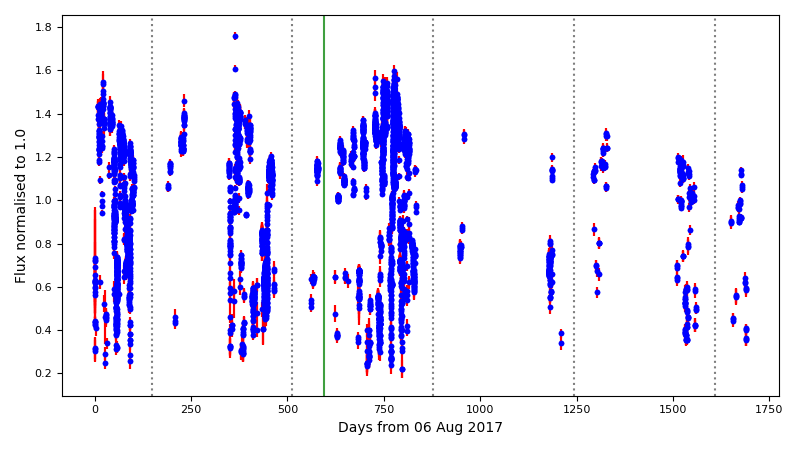
\includegraphics[scale=0.40]{images/remrossallcurve.png} \\
\vspace{-.5cm}
\end{center}
\caption{This shows the total flux after calibration from {\ross}
found in all acceptable images in {\rem}
observations, normalised so that the mean is 1.0. There was a change in
configuration in late March 2019, indicated by the sold vertical green line, but
this occurred 595 days from the start and thus does
not account for any of the shape of the plot
shown. The dotted vertical lines indicate the
start of the years 2018 through to 2022.}\protect\label{fig:rossallcurve}
\end{figure}

\begin{figure}[!htbp]
\begin{center}
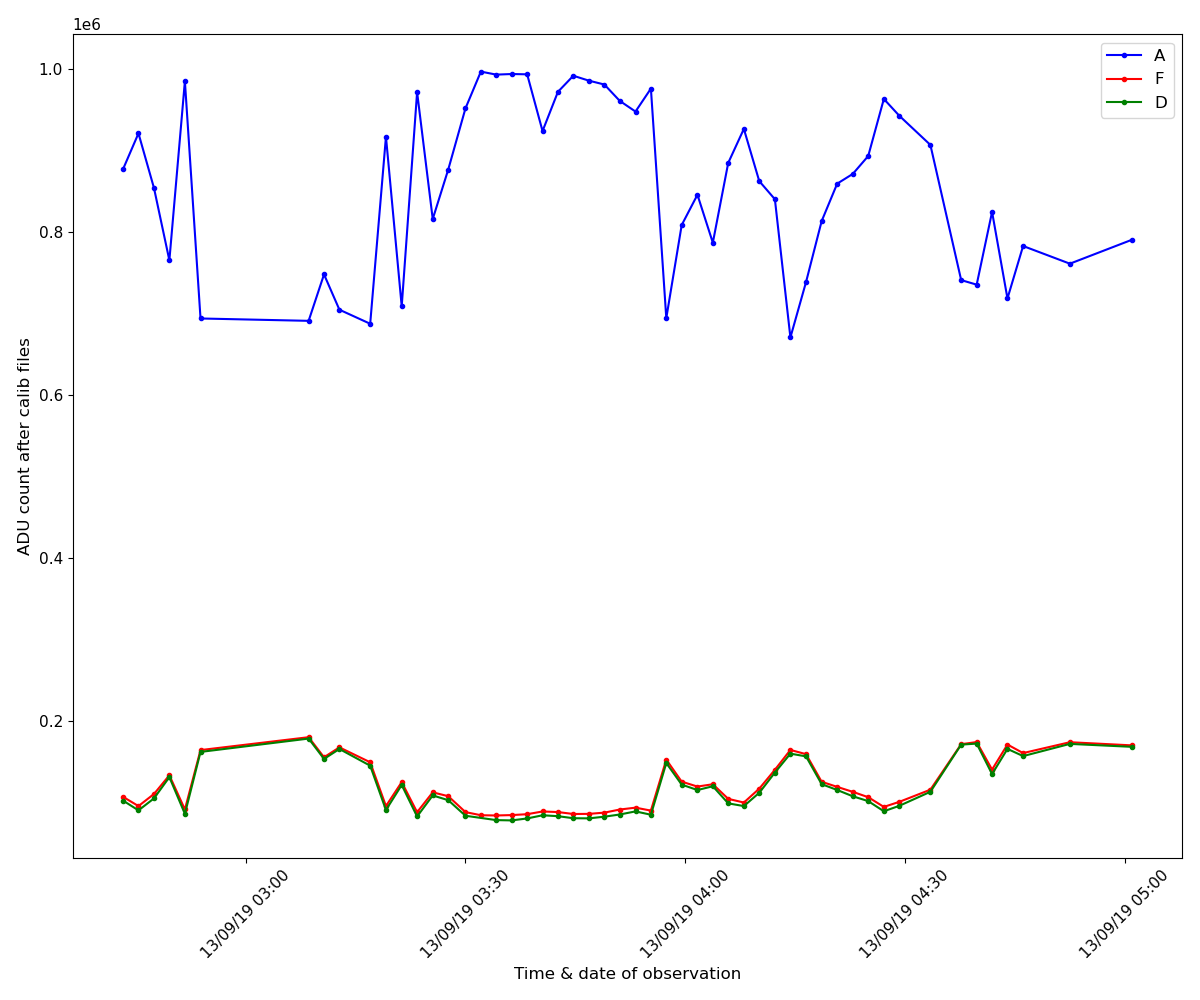
\includegraphics[scale=0.40]{images/all130919.png} \\
\end{center}
\caption{This shows the total flux, with no attempt to calibrate, for {\ross}
and the next two brightest objects visible on 13 September 2019. In this figure
A represents \ross, whilst F and D represent TIC~224752356 and
Gaia~DR3~4075153519816173184 respectively.}\protect\label{fig:2019sept13}
\end{figure}

Observable is the huge jump over the course of about 2 minutes between the
fifth and sixth point on this figure. The flux for {\ross} drops by a quarter in
this time.

Display of the images for the fifth and sixth point on this figure is given in
Fig. \ref{fig:fig5} and Fig. \ref{fig:fig6} respectively. It may be seen that
the sky level has increased by a factor of 3 whilst the maximum flux has reduced
by a about a third. This causes the contrast to be much poorer, with much less
detail.

Concerns about the overall swings are alleviated somewhat, when it seen that
similar swings are observable in observations of {\ross} from other sources, as
shown in Fig. \ref{fig:allsourcelcurve}. However the other sources show an
overall much higher bunching around the mean.

Further work to improve the calculations of the flux is clearly necessary.

\begin{figure}[!htbp]
\begin{center}
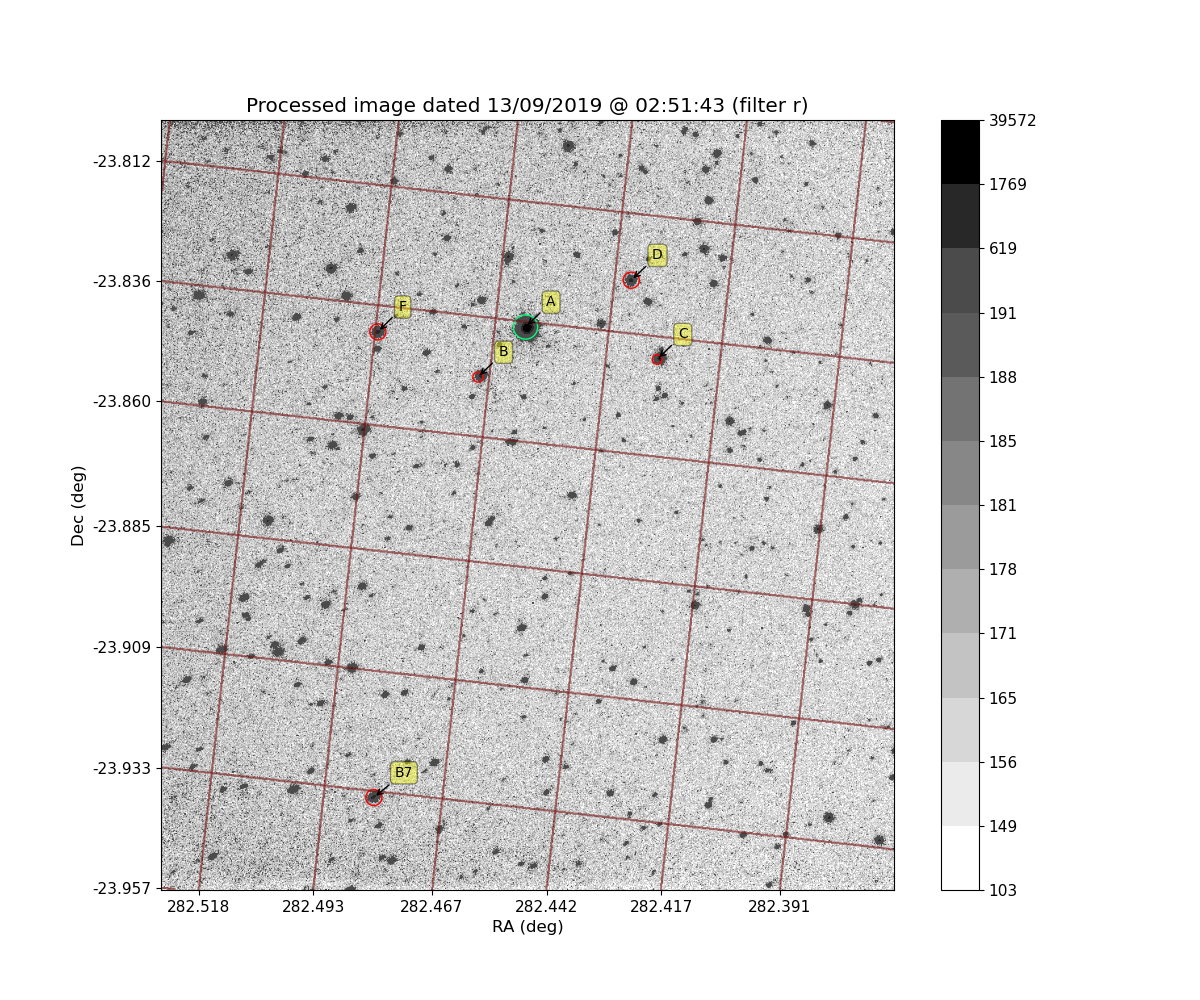
\includegraphics[scale=0.40]{images/fig005.png} \\
\end{center}
\caption{This shows the image for {\ross} on 13
Sept 2019 at 02:51:43 with the 6 strongest sources
identified and labelled,}\protect\label{fig:fig5}
\end{figure}

\begin{figure}[!htbp]
\begin{center}
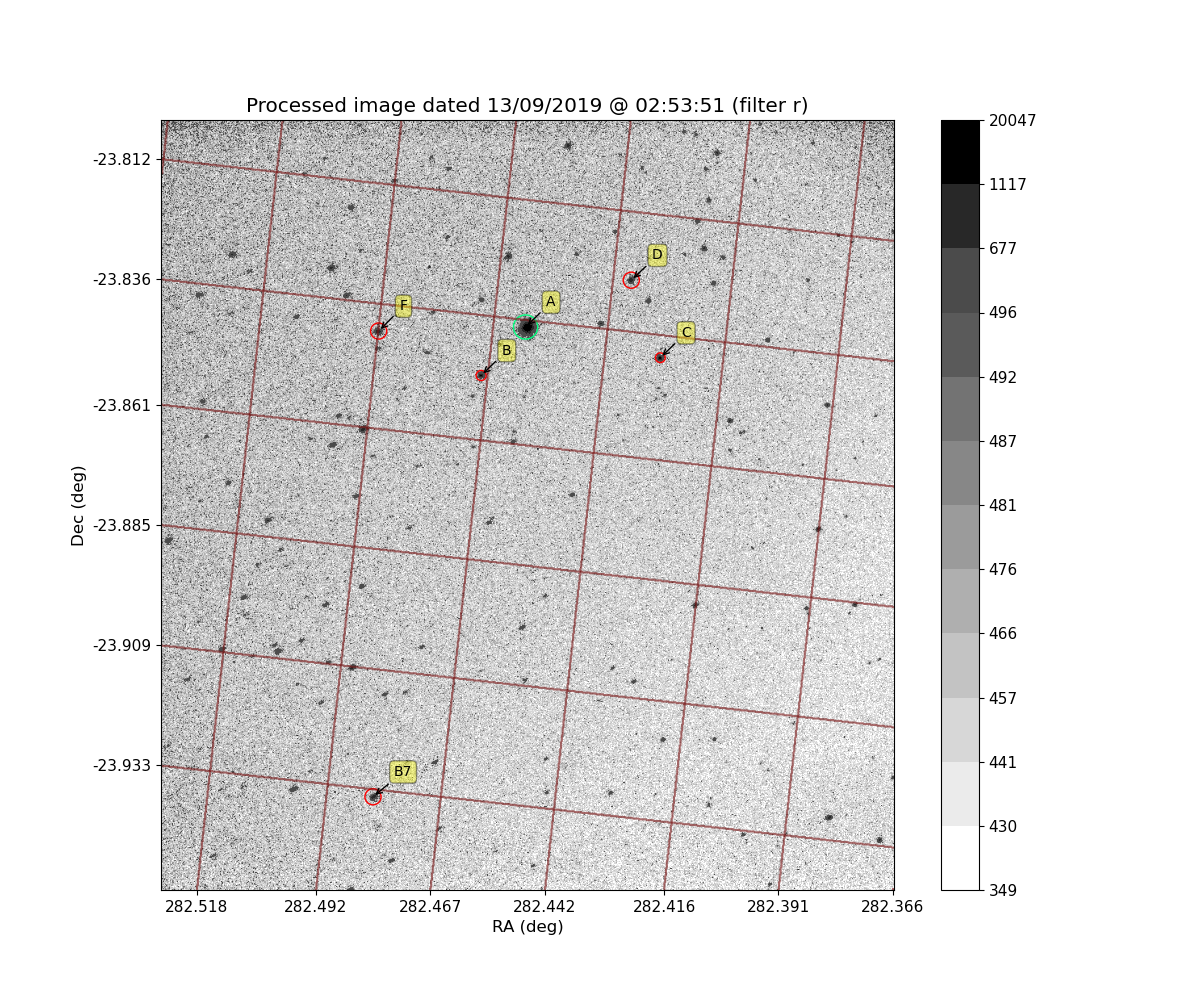
\includegraphics[scale=0.40]{images/fig006.png} \\
\end{center}
\caption{This shows the image for {\ross} on 13
Sept 2019 at 02:53:51 with the 6 strongest sources
identified and labelled,}\protect\label{fig:fig6}
\end{figure}

\begin{figure}[!htbp]
\begin{center}
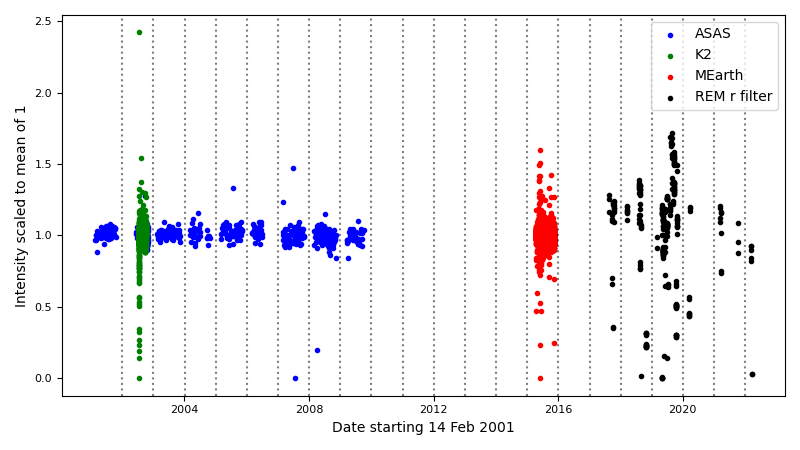
\includegraphics[scale=0.60]{images/comparison.png} \\
\vspace{-.5cm}
\end{center}   
\caption{This figure shows combined data
from ASAS, K2, MEarth and REM, specifically for the \texttt{r} filter,
as blue, green, red and black respectively with the intensity in each normalised
to a mean of 1, i.e. on the same scale, and showing the dates on which each was
taken. The {\rem} light curve is after
calibration by comparison with other objects
in each frame.}\protect\label{fig:allsourcelcurve}
\end{figure}
\clearpage
% \subsection{Set up of pipeline}
% \protect\label{section:pipeline}
%
% A daily routine was set up to interrogate the {\rem} results and load new data
% into the database. The steps were:
%
% \begin{enumerate}
%   \item Load information about new observations into the database. This is just
%   a simple record of information.
%   \item Load FITS files corresponding to the ROSS2 observations of the target
%   objects into the database cache.
%   \item For loaded FITS files, add data about statistics such as maximum and
%   minimum pixel values, mean and standard deviations into the database.
%   \item For database rows corresponding to the targets, compute the barycentric
%   dates and add to the database.
%   \item Identify the target and other objects in the frames and add locations to
%   the database. Mark frame as too poor to use if the target is not found, and
%   less than a given number of reference objects, currently 10, are not found.
%   \item Load FITS files corresponding to daily flat and bias files into the
%   database.
%   \item Load any new master bias and flat files (although these are no longer
%   used).
% \end{enumerate}
%
% The calculation of ADUs for objects is currently done manually when ready, but
% ultimately this will be added to the pipeline. Currently the daily job takes
% about 40 minutes to run.
